\chapter{Robot kinematics}

\section{Parameter framework}
\lipsum[1]

\todo[inline]{
\textbf{Todo}

- Add section about how fluid motion and time dependent variables can be modelled in a computer environment which don't know the concept of time.

- Image of testing program and it's features
}

\subsection{Necessary parameters}
\subsection{Denavit-Hartenberg}
\subsection{Inherent challenges from current framework}

\section{Robot control validation software}

\todo[inline]{
\textbf{Todo}

- Rapid prototyping produced the need for a method to test the calculations more rapid than GeoMod could give.

- This was the intention of the \textit{robot control software}
}

\begin{figure}[h!]
    \centering
    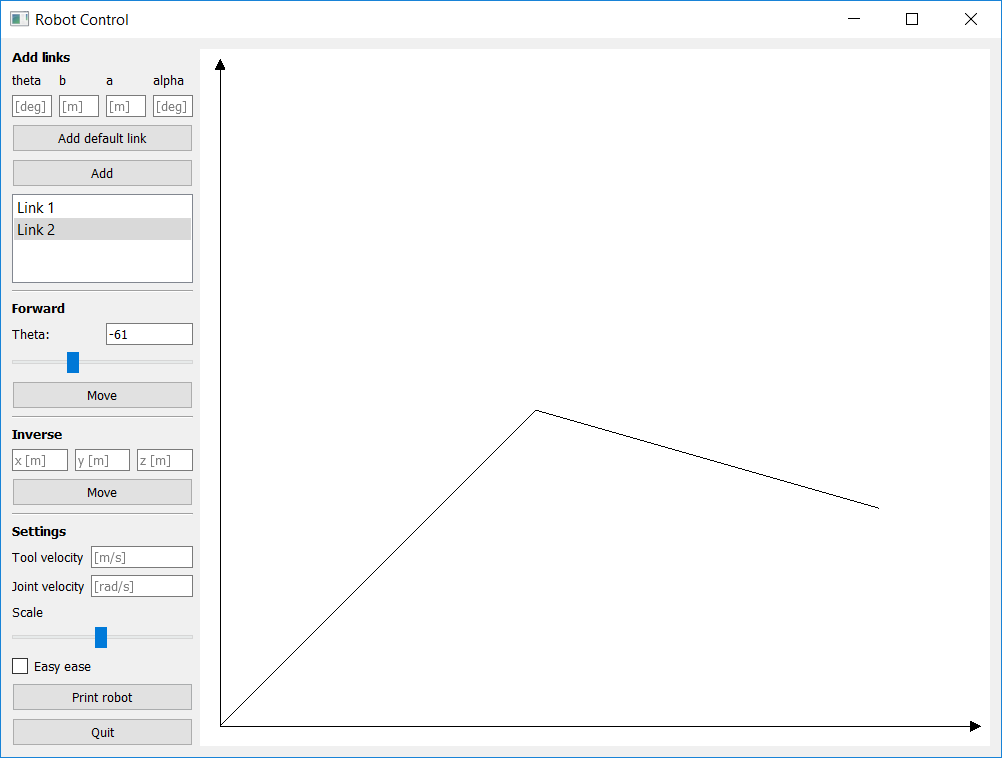
\includegraphics[width=.9\textwidth]{robot_control_interface}
    \caption{\textit{Robot Control} software was used to test the validity of the calculations}
\end{figure}

\begin{figure}[h!]
    \centering
    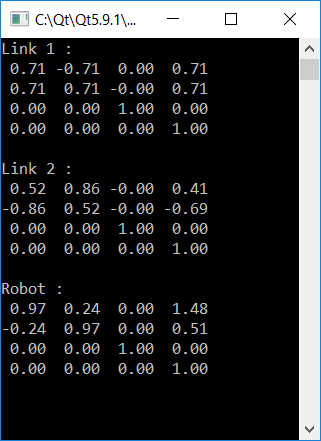
\includegraphics[width=.4\textwidth]{robot_control_console}
    \caption{Console was used to output transformation matrices and other useful information}
\end{figure}

\section{Integration into existing framework}

\todo[inline]{
\textbf{Todo}

- Describe what the current framework was missing and what has been added, highlight differences in class structure

- Show new methods that has been implemented to handle the new parameters
}
\subsection{Jacobian for robot arm}